\chapter{考察}
\section{本システムの有用性と満足度}
表\ref{result01}の結果により,すべての項目の平均値が中央値である3を超えていることから,本手法の有用性が示せたといえる.
しかし,被験者区分別でみると区分Aではデザインの満足度の平均評価値が全体の平均評価値を下回っている.
区分Aの被験者はトランプの知見があり実際にトランプをマジックや,カーディストリーで使用するため,より厳しくデザインを見ていたと考えられる.
自由記述,およびヒヤリングでも,「生成されたデザインをそのまま使うことはない」という意見があった.
また,区分Aの被験者の評価が低くなった要因は初期集団の生成方法にもあると考えられる.
本手法では,既存のデザインから初期集団を生成している.
したがって,既存のデザインに類似していたり,多様性が少なくなったりしたため,トランプに詳しい人にとっては物足りなく感じ,満足度の評価が低くなった考えられる.
しかし,区分Bの被験者の自由記述では「初期集団からいいデザインが多い」という意見が挙がった.
デザインの完成度の高さが,区分Bのデザインに対する満足度の評価値が高かった要因の1つだと考える.
初期集団の生成で多様性を高める方法として,既存の特徴に加え,無作為に生成した図形を組み込むことが挙げられる.
完成度の高さを担保したうえで多様性を高めることができると考えられる.

\section{区分Aと区分Bの被験者の差}
新しいデザインのヒント,アイデアの取得の可否では区分Aの平均評価値が区分Bの平均評価値を上回っていた.
本システムでは,個体集団に同じ図形で細部が異なるデザインが多数生成される.
表\ref{result02}より,区分Aの被験者のほとんどはトランプのデザインを作りたいと考えているとわかる.
デザインは細部の違いで印象が変わることがあり,デザインを作りたいと考えている被験者が印象の変化をヒントやアイデアであると認識した.
したがって,区分Aの平均評価値が区分Bの平均評価値を上回ったと考える.
また,システムの使いやすさに対する評価値でも差が生まれ,区分Aの平均評価値が区分Bの平均評価値を0.8上回った.
結果から,それぞれの被験者の重要視している要素に違いがあると考える.
前述した通り区分A は,トランプのデザインに興味があり,システム全体よりもデザイン単体を見ている.
したがって,無意識に多少の使いにくさを無視しているのだと考えられる.
しかし,システムの使いにくさはユーザの疲労につながり,IGAの重要な要素である個体評価にも影響を与える恐れがある.
使いにくさを助長する要素の一つが集団の個体数の多さであると考えられる.
自由記述では,「生成されたデザインの数が多く評価が疲れる」,「全く同じデザインが多数表示される」との意見が挙がった.
本システムでは,多様なデザインを多く提示するために集団の個体数を30個にしたが,ユーザの負担が大きくなったと考える.
改善策として,構成要素が一定以上同じ個体を排除し,個体を再生成することや,突然変異の確率を高くすることが挙げられる.

\subsection{区分別の評価の高いデザイン}
被験者に自身の中で評価の高かったものを提出させたが,区分Aと区分Bで特色が出た.
それぞれが提出したものの一部を図\ref{A_design}と図\ref{B_design}に示す.
最も大きな違いは色の使い方である.区分Bの被験者のデザインの多くは背景色や線の色が変更されていたのに対して,区分Aの被験者のデザインで両方の色が変更されていたのは1枚だけだった.
区分Aの被験者が普段使用しているトランプは基本的に白い線で描かれており,背景色を含めて2色で構成されているからだと考える.
一方で,区分Bの被験者は色を自分の好みに変えることでデザインの印象を変えていたと考えられる.
% デザインは類似していても色の変更だけでトランプの雰囲気を一変できることがわかった.

\begin{figure}[b!]
    \begin{center}
        \centering
        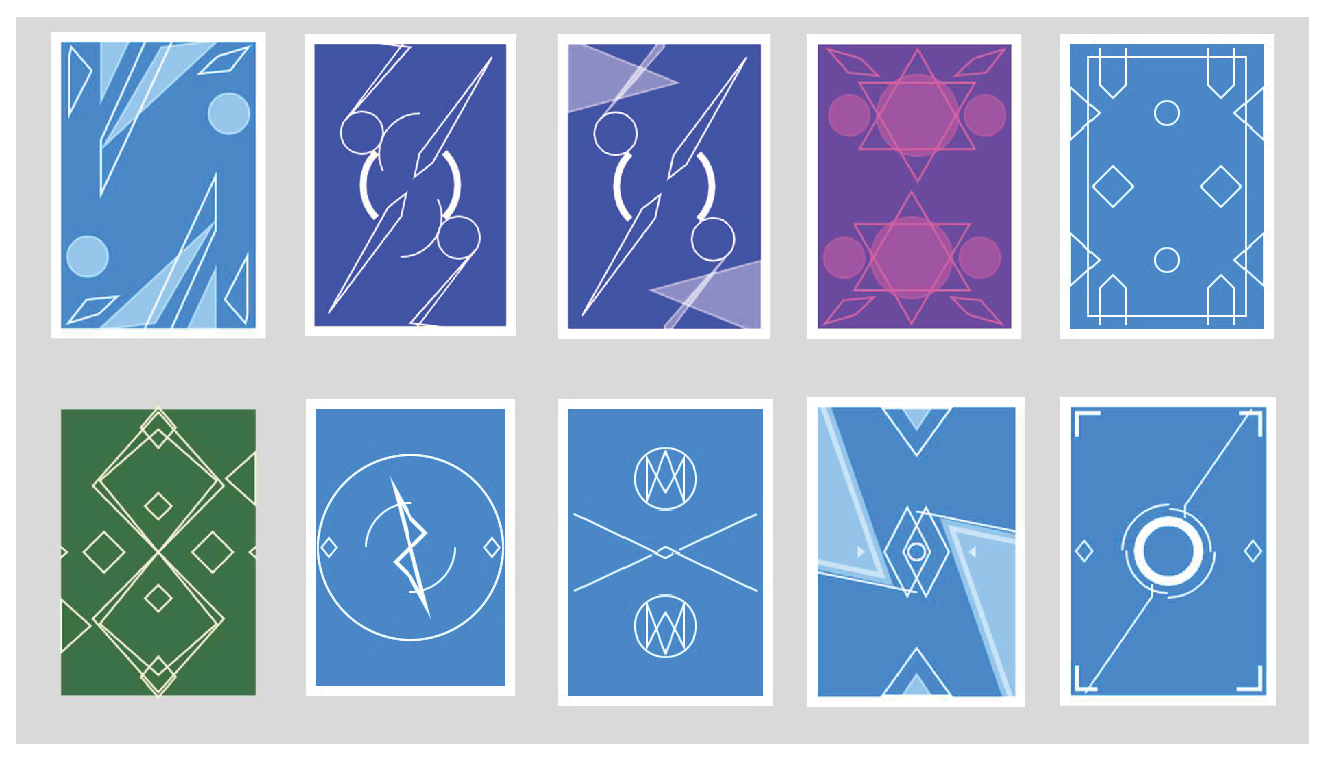
\includegraphics[scale=0.6]{image/playing_cards1.eps}
        \caption{区分Aで評価の高かったデザイン}
        \label{A_design}
    \end{center}
\end{figure}

\begin{figure}[htbp]
    \begin{center}
        \centering
        \includegraphics[scale=0.6]{image/playing_cards4_1.eps}
        \caption{区分Bで評価の高かったデザイン}
        \label{B_design}
    \end{center}
\end{figure}


\section{今後の課題}
個人の感性に基づいたトランプのバックデザイン生成を目的としてシステムを構築した.
本システムによりマジック,カーディストリーで使用するトランプを生成することを想定している.
本システムで生成されたデザインはそのまま使用するには物足りないという結果になった.
一方で,人間では発想しにくいデザインや,細部の異なる多数のデザインを即座に生成することには成功し,デザインからヒントやアイデアを取得することは可能であった.
システムを用いてデザインのヒントやアイデアを与えることに加え,クリエイターのサポートをすることを目的とし,自由記述,ヒアリングの結果をもとに追加機能を提案する.

\subsection{スプレッドとファンを使ったデザインプレビュー}
ヒアリングの結果,生成されたデザインをスプレッド,ファンする機能が必要だとわかった.
スプレッド,ファンとは,第\ref{0201}章で記述した通り,それぞれ扇形,横に長く広げる技法であり,マジックやカーディストリーで頻繁に使われている.
広げた状態を可視化することで,使用されているトランプのイメージをもってデザインすることができると考える.
また,広げる間隔をユーザが変更可能にすることで,配色や線,図形の位置や面積がデザインにどのような影響を与えるかを見ることができると考える.

\subsection{SVG形式でのファイル出力}
表\ref{resultlast}により,ダウンロード機能の有用性は示されている.
しかし,表\ref{free5}からデザインをsvg形式で出力する機能が必要とわかった.
svgとはScalable Vector Graphicsの略であり,画像フォーマットの1つである.
本システムのダウンロード機能ではpng形式の画像をダウンロードできる.
png形式はラスタ形式の画像であり,拡大や縮小をすると画質が劣化する.
対してsvg形式はベクトル形式の画像であり,拡大縮小しても画質が落ちない.
またアニメーションや色,グラデーションの指定なども可能である.
生成したデザインをsvg形式で出力することで,デザインの編集が容易になり,アプリケーションなどでも使えるようになると考える.

\subsection{背景と枠およびボーダーの設定}
表\ref{free5}からデザインに背景や枠を付ける機能が必要とわかった.
今回のシステムでは背景,枠を付ける機能はない.
しかし,ボーダーの太さと共に,背景,枠を変更可能にし,ファンやスプレッドを使ったプレビューを行えば印象が違うものにできると考えられる.
また,ヒアリングで「シンプルなデザインがさみしく感じる」という意見が挙がった.
本来シンプルなデザインには,空間は空いているが複雑なアイコンが使われたり,文字が使われたりすることが多い.
しかし,提案手法では複雑な図形や文字を使うことができないため,背景や枠のデザインを選択可能にすることで,1つの個体で多数のデザインを表現でき,デザイナーやクリエイターの助けになると考えられる.

